\documentclass[9pt]{beamer}
% Created By Gouthaman KG
%~~~~~~~~~~~~~~~~~~~~~~~~~~~~~~~~~~~~~~~~~~~~~~~~~~~~~~~~~~~~~~~~~~~~~~~~~~~~~~
% Use roboto Font (recommended)
\usepackage[sfdefault]{roboto}
\usepackage[utf8]{inputenc}
\usepackage[T1]{fontenc}
%~~~~~~~~~~~~~~~~~~~~~~~~~~~~~~~~~~~~~~~~~~~~~~~~~~~~~~~~~~~~~~~~~~~~~~~~~~~~~~

%~~~~~~~~~~~~~~~~~~~~~~~~~~~~~~~~~~~~~~~~~~~~~~~~~~~~~~~~~~~~~~~~~~~~~~~~~~~~~~
% Define where theme files are located. ('/styles')
\usepackage{styles/fluxmacros}
\usefolder{styles}
% Use Flux theme v0.1 beta
% Available style: asphalt, blue, red, green, gray 
\usetheme[style=asphalt]{flux}
%~~~~~~~~~~~~~~~~~~~~~~~~~~~~~~~~~~~~~~~~~~~~~~~~~~~~~~~~~~~~~~~~~~~~~~~~~~~~~~

%~~~~~~~~~~~~~~~~~~~~~~~~~~~~~~~~~~~~~~~~~~~~~~~~~~~~~~~~~~~~~~~~~~~~~~~~~~~~~~
% Extra packages for the demo:
\usepackage{booktabs}
\usepackage{colortbl}
\usepackage{ragged2e}
\usepackage{schemabloc}
\usepackage{hyperref}
\usebackgroundtemplate{

\includegraphics[width=\paperwidth,height=\paperheight]{assets/background.jpg}}%change this to your preferred background for the presentation.
%~~~~~~~~~~~~~~~~~~~~~~~~~~~~~~~~~~~~~~~~~~~~~~~~~~~~~~~~~~~~~~~~~~~~~~~~~~~~~~

%~~~~~~~~~~~~~~~~~~~~~~~~~~~~~~~~~~~~~~~~~~~~~~~~~~~~~~~~~~~~~~~~~~~~~~~~~~~~~~
% Informations
\title{TEMPLATE}
\subtitle{WITH CUSTOM BACKGROUND AND LOGO}

\author{GKG }
\institute{}
\titlegraphic{assets/gkg.png} %change this to your preferred logo or image(the image is located on the top right corner).
%~~~~~~~~~~~~~~~~~~~~~~~~~~~~~~~~~~~~~~~~~~~~~~~~~~~~~~~~~~~~~~~~~~~~~~~~~~~~~~

\begin{document}

% Generate title page
\titlepage

\begin{frame}

 \frametitle{TABLE OF CONTENTS}
 \tableofcontents
\end{frame}

\section{EXAMPLE 1} %the content in the section will be displayed in the table of contents
\begin{frame}{EXAMPLE 1}%the content in the frame will be displayed as the title of the page
"Lorem ipsum dolor sit amet, consectetur adipiscing elit, sed do eiusmod tempor incididunt ut labore et dolore magna aliqua. Ut enim ad minim veniam, quis nostrud exercitation ullamco laboris nisi ut aliquip ex ea commodo consequat. Duis aute irure dolor in reprehenderit in voluptate velit esse cillum dolore eu fugiat nulla pariatur. Excepteur sint occaecat cupidatat non proident, sunt in culpa qui officia deserunt mollit anim id est laborum."
    
\end{frame}

\section{EXAMPLE 2}
\begin{frame}{EXAMPLE 2}
\begin{itemize}

  \setlength\itemsep{1em}  %increase the space between items.
  
    \item "Lorem ipsum dolor sit amet, consectetur adipiscing elit, sed do eiusmod tempor incididunt ut labore et dolore magna aliqua. Ut enim ad minim veniam, quis nostrud exercitation ullamco laboris nisi ut aliquip ex ea commodo consequat. Duis aute irure dolor in reprehenderit in voluptate velit esse cillum dolore eu fugiat nulla pariatur. 
    
    \item Excepteur sint occaecat cupidatat non proident, sunt in culpa qui officia deserunt mollit anim id est laborum."
\end{itemize}
\end{frame}

\section{EXAMPLE 3}
\begin{frame}{EXAMPLE 3}
    \begin{table}[H]
	\begin{center}
    \begin{tabular}{l l l l l l l}
    \toprule
    \multicolumn{7}{c}{Moreira Muir Strategy Results starting 1946} \\
    \midrule
             Statistic &     Mkt$^{\sigma}$ &     SMB$^{\sigma}$ &    HML$^{\sigma}$ &     Mkt &    SMB &     HML \\
    \midrule
  Avg Total Return &    0.83 &    0.24 &    0.57 &    0.86 &   0.35 &    0.62 \\
 Avg Excess Return &    0.51 &   -0.09 &    0.25 &    0.53 &   0.03 &    0.29 \\
 Std Excess Return &    4.25 &     2.8 &    2.65 &    4.25 &   2.81 &    2.65 \\
  Sharpe Geometric &    0.41 &   -0.11 &    0.32 &    0.44 &   0.03 &    0.38 \\
          Skewness &    0.17 &   -0.98 &     0.3 &   -0.54 &    0.5 &    0.45 \\
          Kurtosis &    5.48 &     9.6 &    5.07 &    1.79 &   6.61 &    2.92 \\
               Min &  -20.19 &  -20.73 &  -15.38 &  -23.25 &  -15.6 &  -11.39 \\
               Max &   28.08 &   15.96 &   16.24 &   16.16 &  22.19 &   14.28 \\
             alpha &    1.97 &    -1.1 &    0.68 &    -0.0 &   -0.0 &    -0.0 \\
       Factor Beta &    0.69 &    0.68 &    0.69 &     1.0 &    1.0 &     1.0 \\
               PSR &    0.27 &     0.0 &    0.04 &     0.5 &    0.5 &     0.5 \\
    \bottomrule
    \end{tabular}
	\caption{Short caption...}
    \label{tab:MMresults}
    \end{center}
    \end{table}
\end{frame}


\section{EXAMPLE 4}
\begin{frame}{EXAMPLE 4}
   \begin{figure}[h]
			\centering
			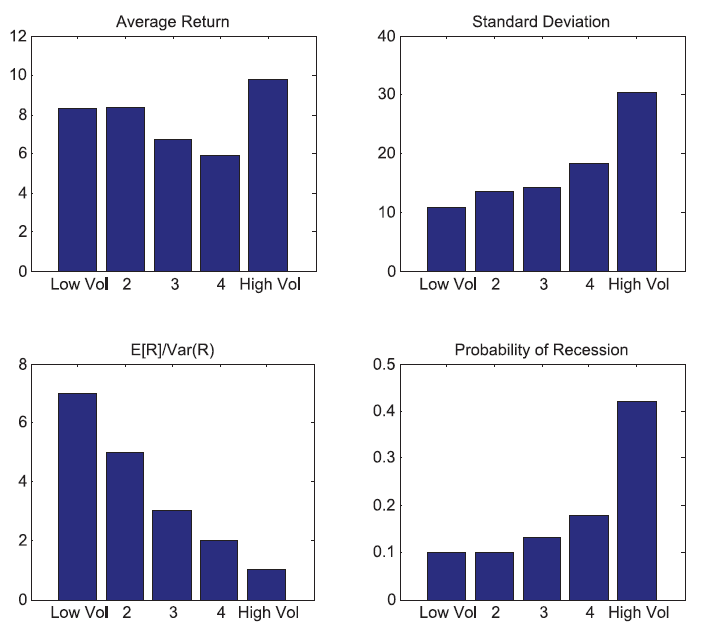
\includegraphics[width = 0.7\textwidth]{img/MM.PNG}
            \label{fig:MManalysis}
	\end{figure}
\end{frame}
    

\end{document}